\section{PuzzleScript Design}
\label{sec:puzzlescript}
This design is based on observed code and behaviours from the original JavaScript implementation. PuzzleScript does not have an official design document\footnote{\url{https://groups.google.com/g/puzzlescript/c/UBe9M8QP-rk}}. Part of the design was formalized by Vermeulen\cite{vermeulenautomated}.

A PuzzleScript file stores exactly one PuzzleScript game, there are no ways to store multiple games in a file or to split up one game into multiple files. A game is made up of a prelude and multiple sections.

A prelude is a list of lines before the first section. Each line contains at most two tokens, a key and a value. The pairs allow the developer to modify the way the engine works or the visual aspect of their game. Some keys do not require a value. Values can be a string (a list of tokens displayed literally), a numeral (int or float) or a member from an enumerator. 

A full list of possible prelude keys and their values is already documented in PuzzleScript's user guide\footnote{\url{https://www.puzzlescript.net/Documentation/prelude.html}}. 

% list of key-value pair lines which allow the developer to slightly modify how the engine runs and the visual aspects of sprites.

Following the prelude are the sections, in the JavaScript implementation they have a specific order because the code is checked as it is parsed. So the static checker only knows what has been parsed so far. It is unknown whether that order exists in the theoretical design of PuzzleScript. A game is made up of exactly seven sections that cannot be duplicated and that must be present if only empty. A section is made up of a header stating the section name and optionally prefixed/suffixed by a line of \texttt{=} from the other sections. Everything after that and until the next section header begins is considered the section's content and must follow the syntax rules assigned to that section. The order of the sections is as follows:
\begin{itemize}
    \item Objects: Defines all the objects to be used in the game
    \item Legend: Create shorthand links between symbols and objects to allow properties, aggregation of objects and tilemap creation.
    \item Sounds: Defines handlers to play sounds when certain events happen
    \item Layers: How objects interact with each other movement-wise, whether they can stack or if they collide
    \item Rules: How objects interact, what happens when certain items are next to each other or if a player tries to move into a certain item
    \item WinConditions: Defines victory conditions for the level
    \item Levels: List of tilemaps and messages that represent the different rooms the player will explore
\end{itemize}

Everything links back to Objects, objects are placed on levels, specified in rules and win conditions albeit sometimes through the use of legends. An object is made up of a name, an optional symbol for a legend, a list of colours and optionally a 5x5 sprite. Colours are either an HTML colour code or a colour keyword from the selected palette. The colour palette available is decided by the developer in the prelude from a wide range. If no sprite is provided then the object appears as a solid 5x5 block of the first colour defined. The sprite is a 5x5 tilemap of where the \texttt{.} represent a transparent pixel and numbers from \texttt{0-9} represents a coloured pixel based on the index of the coloured list. As can be seen in Figure \ref{fig:object_code}, \texttt{0} represent blue because it is the first colour in the list of colours defined for that objects.

The name and legend of the object can be almost any character, although choosing certain characters can be an issue in other sections. For example, naming an object any of the directional arrows is a legal move, but it raises a warning and means that you cannot use the object name in the Rule Section. Sometimes, using reserved keywords for objects still works but can confuse the syntax highlighter and will definitely confuse the reader of the code.

\begin{figure}
    \centering
    \begin{lstlisting}[language=PuzzleScript]
        CRATE C
        BLUE RED
        00000
        0...0
        0...0
        0...0
        00000
    \end{lstlisting}
    \caption{An Object}
    \label{fig:object_code_old}
\end{figure}

Legends allow the developer to create shorthand references to one or more objects. They are made up of a list of symbols followed by an 'and'/'or' separated list of object names or other references. References cannot mix the 'and' and 'or' separators and cannot make use of legends that use the other separator. 'Or' separated legends are called properties and serve to reference multiple objects at once in rules, victory conditions or sounds. 'And' separated legends are called aggregates and can be used in rules and levels to define items stacked on top of each other. Legends made up of a single object are aliases, they perform the same task as properties but can also be used to create level tilemaps.

\begin{figure}
    \centering
    \begin{lstlisting}[language=PuzzleScript]
        Obstacle = Crate or Wall
        P = Player
        O = Target And Crate
    \end{lstlisting}
    \caption{Some legends}
    \label{fig:legend_code_old}
\end{figure}

Sound is a very flexible system that allows you to assign sounds to certain interactions or triggers when rules happen. They are made up of either a reference or a sound keyword (SFX[0-10]) followed by a list of filters (moving, stationary) and finally a sound seed. Sound seeds are generated by the editor. The sound system is quite well explained in PuzzleScript's user documentation\footnote{\url{https://www.puzzlescript.net/Documentation/sounds.html}}

Layers are a list of objects or properties separated by an optional comma (\texttt{,}) or white space. Objects on the same line cannot stack with one another. All objects must be referenced in this section, either directly or through a legend. This restriction is put in place so that the developer does not accidentally spawn an item that has not been defined collision wise. Placing an object in multiple layers is a legal move but raises a warning and can have unintended consequences.

\begin{figure}
    \centering
    \begin{lstlisting}[language=PuzzleScript]
        Crate, Player, Wall
    \end{lstlisting}
    \caption{A Layer}
    \label{fig:layer_code_old}
\end{figure}

Rules are the heart of PuzzleScript. A rule is made of a series of prefixes that affect the whole rule, a left side "pattern" and a right side "replacement". The left side must contain at least one rule part, the right side must contain 0 or exactly the same number of rule parts as the left side.  Rule parts start with a \texttt{[} and ends with a \texttt{]}. Within a rule part, there are a certain number of rule sections, each rule part on the right must have the same number of sections as the equivalent rule part on the left. Sections of a rule part are separated by \texttt{|}. Each section is made up of object references that can stack and each object can have one modifier applied to it. Modifiers allow checking for special matches such as moving objects or the absence of an object. Each section represents an adjacent cell, either vertical or horizontal. Rules can be marked as "late" which means they will run in a second phase after the player movement has been processed. More information on the rules can be found in PuzzleScript's user manual\footnote{\url{https://www.puzzlescript.net/Documentation/rules.html}}. This design documentation is focused on the design restriction that cannot be found there.

\begin{figure}
    \centering
    \begin{lstlisting}[language=PuzzleScript]
        [ >  Player | Crate ] -> [  >  Player | > Crate  ]
        late [ Crate | Crate | Crate ] -> [ | |]
    \end{lstlisting}
    \caption{A few Rules}
    \label{fig:rule_code_old}
\end{figure}

WinConditions are a simple way to create a victory condition for levels. In the current implementation, all conditions need to be met for a level to be won. A condition is made up of a keyword and a legend or object followed by an optional \texttt{on} keyword that defines another object to be stacked upon. The possible keywords are \texttt{Some}, \texttt{No} and \texttt{All}. \texttt{Some} is true if any of the objects are present on the level, when combined with the \texttt{on} keyword it is true if at least one of either object is stacked on the other.

It is important to note that the "OBJECT1 on OBJECT2" syntax is misleading. For example, in the case of \texttt{All Crate on Target} what this means is that there cannot be a target that is not on the same XY coordinate\footnote{We define "stacked" as being on the same XY coordinate as PuzzleScript does not require for a specific item to be on top, as such, an item can still be on another item even if that first item is actually under.} as a Crate. However, from a natural language point of view, one would assume the contrary, that each Crate must be on the same XY as a Target. This kind of distinction is important when there is more of one object than of the other. For example, if there are four Target and three Crate then the level is impossible to win.

\begin{figure}
    \centering
    \begin{lstlisting}[language=PuzzleScript]
        Some target on crate
        No Player
        All oranges on plates
    \end{lstlisting}
    \caption{Some win conditions}
    \label{fig:conditions_code_old}
\end{figure}

Level are tilemaps made up of symbols, the tilemaps can have any width or length but every line must be the same length. The Level section also accepts messages which are the keyword \texttt{message} and a set of words that will appear between the two levels. Each symbol on a tile map must reference either a single object through the use of their name (if the name is only one symbol long) or of the object legend or it must reference an aggregation of objects representing multiple objects in the same place.

\begin{figure}
    \centering
    \begin{lstlisting}[language=PuzzleScript]
        message Level 1: Beginnings
    
        ####..
        #.O#..
        #..###
        #@P..#
        #..*.#
        #..###
        ####..
    \end{lstlisting}
    \caption{A message and a level}
    \label{fig:level_code_old}
\end{figure}

\subsection{JavaScript Implementation}
This part only refers to the official implementation of PuzzleScript written by the original developer, Stephen Lavelle, in JavaScript.

The JavaScript implementation of the PuzzleScript engine is broken down into three phases:
\begin{itemize}
    \item Parsing: This phase reads the source code and checks the validity of the code it parsed
    \item Compiling: This phase transforms the code into JavaScript data structures that the PuzzleScript engine can read. This also involved transforming the rules into JavaScript functions. This section also checks some of the compiled code for validity.
    \item Engine: This runs the engine by waiting for player input when the game screen is focused.
\end{itemize}

The source code directory is made up of 27 files which add up to 15,000 lines of code, calculated using \textbf{cloc}\footnote{\url{http://cloc.sourceforge.net/}}. A lot of these are used to store code that provides additional functions or very niche parts of the engine. Looking through the code, we have identified three files that take care of the majority of the workload. These are:
\begin{itemize}
    \item parser.js: 1065 lines, takes care of the Parsing phase.
    \item compiler.js: 2350 lines, takes care of the Compiling phase
    \item engine.js: 2405 lines, takes care of the Engine phase
\end{itemize}

So the core of PuzzleScript itself totals 5820 lines of code. 

Part of the official implementation is also the in-browser IDE, which is implemented using the versatile library CodeMirror\footnote{\url{https://codemirror.net/}}. This is the same library implemented by Rascal's web development library salix. 

The IDE provides comprehensive syntax colouring which also adapts to its context. Sprite pixels that represent a colour will appear as that colour. Syntax colouring will fail if the syntax is incorrect, reporting similar errors to the static checker. 

\begin{figure}[h]
    \centering
    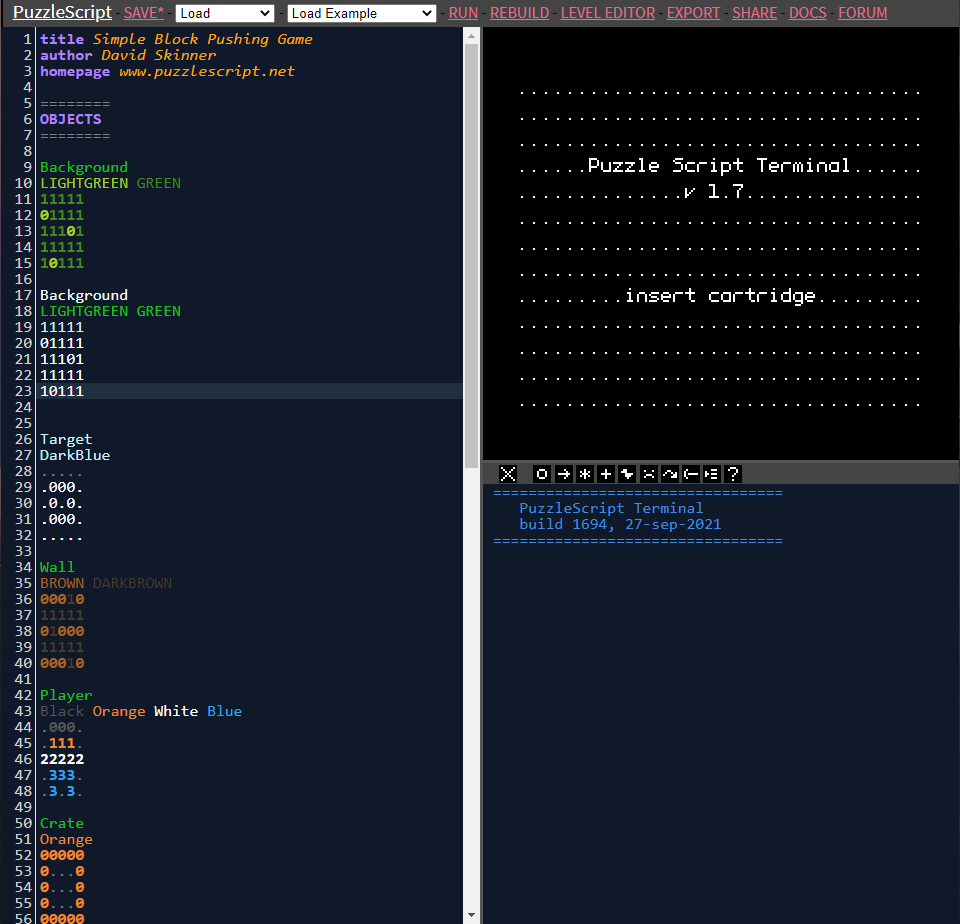
\includegraphics[width=1\textwidth]{images/PuzzleScript_IDE.png}
    \caption{PuzzleScript's browser IDE}
    \label{fig:browser_ide_old}
\end{figure}

Once the user presses "Run" the game will be compiled, errors will appear in the bottom right and the title screen for the game will appear in the top right. The top bar of the IDE provides a lot of additional options for sharing and exporting the game into a standalone application alongside helpful links for seeking support. 

The implementation displays error messages as they are detected and aborts compilation if a certain threshold is reached. The threshold is necessary because of the possibility of an error cascade, if there was no threshold a high number of ghost errors might be displayed, making it harder to fix the true issues. With the threshold, the developer is encouraged to address errors a little bit at a time, allowing the static checker to clear up any ghost errors.

User inputs are context-sensitive, if the user presses an arrow key while focused on the editor it will move their cursor text if they do the same with a focus on the game it will attempt to move their character. The IDE does not have a contextual right-click menu.

% One of the main weaknesses we discovered in the JavaScript implementation is the lack of segmentation of the various phases normally expected from an engine. This meant that a single error would create a fault in the parsing process, causing the remaining lines to be marked as invalid. This would usually result in a couple of lines of error before the compiler aborts to avoid an overflow. In practice, the weakness would mean that only one real error would be reported each time you ran the compiler in charge of checking the validity of the code. 

\subsection{Design and Implementation Shortcomings}
PuzzleScript is an incredibly flexible language, both in design and through implementation. However, this flexibility causes certain corner cases that make it quite hard to formalize the grammar. Instead of declaring certain characters and tokens as globally reserved keywords, PuzzleScript took the approach of having a section-specific list of reserved keywords. As an example, specifying the legend for an item as \textbf{]} is allowed, however, the trade-off is that you cannot use that legend to reference the item in the Rules section, since \textbf{[]} are reserved symbols in that section. You can still use it to reference an object in a tilemap. This is made possible by the technical implementation of PuzzleScript's parse which is line-based and handcrafted. This classes PuzzleScript's grammar as context-sensitive.

The question we pose now is whether or not this extra flexibility is worth it. The JavaScript implementation raises a warning when it occurs but functions perfectly well. This extra flexibility makes it hard to formalize the grammar since section-specific keywords are not a common design pattern. Few languages are pure context-free grammars but PuzzleScript is especially context-sensitive. 

The tightly coupled phases make it hard to extend the codebase. In addition, any extension needs to take care of the full process, from adding it to the syntax colouring to displaying log messages. There are no "general" functions that can be simply provided as a set of instructions for extensions. 

Rules, the heart of PuzzleScript, are the hardest part of the code to read. They are compiled into PuzzleScript functions using metaprogramming, which essentially means that a great part of the engine does not exist until runtime. Because JavaScript is dynamically typed it makes it hard to understand what is being passed to these functions. 

In the JavaScript implementation, parsing is one of the two phases and is done simultaneously with error checking. This can very easily cause errors to cascade since any error also throws the parser off as can be seen in Figure \ref{fig:error_cascade}. This means that errors are ephemeral and only exist for the single cycle during which they are generated, after that there is no way for any plugin to access them. The graphics engine are similarly coupled, graphics are generated as rules are applied and objects have methods for generating graphics directly attached to them. This can make it hard to extend PuzzleScript as a game does not exist only as a data structure but also partly as a set of graphics.

\begin{figure}[!t]
    \centering
    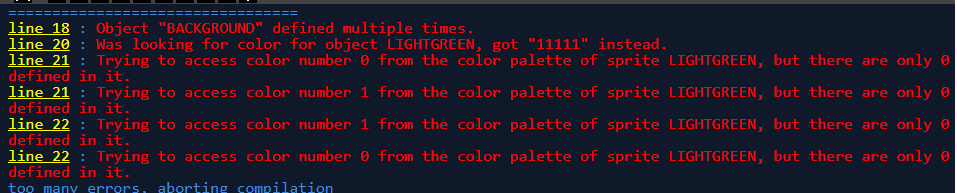
\includegraphics[width=1\textwidth]{images/Example_errors_current.png}
    \caption{A single error causes a cascade of ghost errors}
    \label{fig:error_cascade_old}
\end{figure}

The IDE itself is simple, offering syntax colouring and printing the errors, its real power comes from the engine itself which allows it to run games with great performance directly in the browser.

The conclusion is that PuzzleScript is a complex language that appears simple to the users which is implemented in order to prioritise performance and portability at the cost of extensibility and maintainability.
